\selectlanguage{italian}

\section{Radioattività}

I primi indizi verso la radioattività sono derivati dalla rilevazione dei raggi X: questi sono onde elettromagnetiche, ovvero fotoni, generate da transizioni di elettroni tra livelli energetici ($ \Delta E_e = \hbar \omega $); questi dunque non sono processi nucleari, dato che avvengono all'interno della nube elettronica dell'atomo.\\
Quando si parla di radioattività in senso stretto, però, si fa riferimento ai decadimenti dei nuclidi.

\subsection{Decadimenti radioattivi}

I decadimenti radioattivi sono processi in cui un nuclide stabile raggiunge una configurazione con energia più bassa emettendo spontaneamente radiazione.\\
Utilizzando un campo magnetico, Rutherford riuscì a distinguere tre tipologie di radiazione, e dunque di decadimenti radioattivi:
\begin{enumerate}
  \item decadimento $ \alpha $, in cui la radiazione è costituita da un nucleo di $ \ch{^4_2 He} $ ed è poco penetrante, coinvolge l'interazione elettromagnetica e quella forte;
  \item decadimento $ \beta^{\pm} $, in cui la radiazione è costituita da un $ e^{\pm} $ ed è mediamente penetrante, coinvolge l'interazione debole:
    \begin{itemize}
      \item decadimento $ \beta^- $: $ n \rightarrow p^+ + e^- + \bar{\nu}_e $;
      \item decadimento $ \beta^+ $: $ p^+ \rightarrow n + e^+ + \nu_e $;
    \end{itemize}
  \item decadimento $ \gamma $, in cui la radiazione è costituita da un fotone con energia dell'ordine delle decine di MeV, dunque estremamente penetrante.
\end{enumerate}
A questi si aggiunge la cattura elettronica, un decadimento in cui un nuclide proton-rich cattura un elettrone dalle shell interne dell'atomo, seguendo la reazione $ p^+ + e^- \rightarrow n + \nu_e $, emettendo raggi X a seguito del rimpiazzo dell'elettrone interno con uno dalle shell esterne.

\subsection{Energy balance}

Un decadimento radioattivo può essere visto come un caso particolare di reazione nucleare; è quindi possibile definire il $ Q $-value del decadimento come la differenza di energia a riposo (massa) tra reagenti (nuclide instabile) e prodotti, così da poter stabilire qualora esso sia possibile, ovvero spontaneo, con la condizione $ Q > 0 $.\\
In particolare, si definiscono i $ Q $-values dei seguenti decadimenti:
\begin{enumerate}
  \item decadimento $ \alpha $: $ Q_{\alpha} \equiv \left[ M(Z,A) - M(Z-2,A-4) - m(\ch{^4_2 He}) \right] c^2 $;
  \item decadimento $ \beta^- $: $ Q_{\beta^-} \equiv \left[ M(Z,A) - M(Z+1,A) - m_e \right] c^2 $;
  \item decadimento $ \beta^+ $: $ Q_{\beta^+} \equiv \left[ M(Z,A) - M(Z-1,A) - m_e \right] c^2 $;
  \item electron capture: $ Q_{e} \equiv \left[ M(Z,A) + m_e - M(Z-1,A) \right] c^2 $;
\end{enumerate}
Si vede subito che $ Q_e > Q_{\beta^+} $: di conseguenza, nell'electron capture i prodotti di decadimento hanno maggior energia cinetica disponibile, inoltre ci sono dei casi in cui può avvenire l'electron capture ma non il decadimento $ \beta^+ $.

\subsection{Radioactive decay law}

Il processo di decadimento ha natura aleatoria, dunque va trattato in maniera statistica.\\
Il numero di decadimenti al secondo è proporzionale al numero di nuclidi radioattivi:
\begin{equation}
	- \frac{dN}{dt} = \lambda N(t)
	\label{eq:2.1}
\end{equation}
Si trova quindi la legge di decadimento esponenziale:
\begin{equation}
	N(t) = N_0 e^{-\lambda t}
	\label{eq:2.2}
\end{equation}
Si definisce inoltre il decay rate (o activity) come $ A(t) \defeq \lambda N(t) $, misurato in Bequerel $ 1\,\text{Bq} = 1 \,\text{decay}/\text{s} $ o in Curie $ 1\,\text{Ci} = 3.7\cdot10^{10}\,\text{Bq} $ (activity di $ 1\,\text{g} $ di radio). Si definiscono inoltre la half-life $ t_{1/2} \equiv \frac{\ln 2}{\lambda} $ e la vita media $ \tau = \frac{1}{\lambda} $ rispettivamente come il tempo dopo il quale il campione si è ridotto di $ \frac{1}{2} $ e di $ \frac{1}{e} $: si ha $ t_{1/2} \approx 0.693 \tau < \tau $.\\
Per i decay rates si trova facilmente che, definendo $ A_0 \equiv \lambda N_0 $:
\begin{equation}
	A((n+1)t) = A(t) \left( \frac{A(t)}{A_0} \right)^n
	\label{eq:2.3}
\end{equation}
Nel caso di una miscela di radioisotopi, è possibile risalire alle singole costanti di decadimento nel caso in cui le vite medie siano molto diverse, poiché quando la specie con la $ \tau $ più corta è completamente decaduta si può misurare direttamente la $ \lambda $ dell'altra specie, per poi risalire a quella della prima tramite la differenza delle activities.

\subsubsection{Decay branches}

Può capitare che lo stesso nuclide radioattivo possa decadere in due o più modi differenti, detti decay branches: detta $ \lambda_k $ la costante di decadimento parziale della $ k $-esima branch, nel caso di $ n $ branches si ha:
\begin{equation}
	\lambda \equiv \lambda_1 + \dots + \lambda_n
	\label{eq:2.4}
\end{equation}
e questa costante totale è l'unica che si osserva, anche quando si rileva una sola delle branches. Si definiscono i branching ratios come $ B_k \defeq \frac{\lambda_k}{\lambda} $.

\subsubsection{Decay chains}

Spesso, in un decadimento radioattivo, capita che anche i prodotti siano radiaottivi: ciò dà vita ad una catena di decadimenti $ N_1 \xrightarrow{\lambda_1} N_2 \xrightarrow{\lambda_2} N_3 \dots $, dove le $ \lambda_k $ sono diverse tra loro.\\
Una decay chain è descritto da un sistema di coupled differential equations. Nel caso, ad esempio, di un doppio decadimento (quindi con prodotto $ N_3 $ stabile):
\begin{equation}
	\begin{cases}
		\dot{N}_1 = - \lambda_1 N_1 \\
		\dot{N}_2 = \lambda_1 N_1 - \lambda_2 N_2 \\
		\dot{N}_3 = \lambda_2 N_2
	\end{cases}
	\quad\Longrightarrow\quad
	\begin{cases}
		N_1(t) = N_0 e^{-\lambda_1 t} \\
		N_2(t) = \frac{\lambda_1}{\lambda_1 + \lambda_2} N_0 \left( e^{-\lambda_1 t} - e^{-\lambda_2 t} \right) \\
		N_3(t) = \frac{\lambda_1 \lambda_2}{\lambda_1 + \lambda_2} N_0 \left( \frac{1 - e^{-\lambda_1 t}}{\lambda_1} - \frac{1 - e^{-\lambda_2 t}}{\lambda_2} \right)
	\end{cases}
	\label{eq:2.5}
\end{equation}
La soluzione generale al caso di $ n $ decadimenti è dato dall'\textit{equazione di Bateman}:
\begin{equation}
	N_k(t) = \sum_{i = 1}^{k} \left[ N_0^{(i)} \left( \prod_{j = 1}^{k-1} \lambda_j \right) \left( \sum_{j = i}^{k} \frac{e^{-\lambda_j t}}{\prod_{p=i, p\neq j}^{k} (\lambda_p - \lambda_j)} \right) \right]
	\label{eq:2.6}
\end{equation}

\paragraph{Equilibrio radioattivo} Si parla di equilibrio radioattivo quando la specie radioattiva madre e quella figlia hanno la stessa attività, ovverosia quando la specie figlia decade allo stesso rate a cui è prodotta. In una decay chain, l'equilibrio radioattivo può instaurarsi tra ciascuna coppia di nuclidi della catena: la condizione generale da soddisfarre è che $ (t_{1/2})_{\text{madre}} > (t_{1/2})_{\text{figlia}} $.\\
In particolare, si parla di:
\begin{enumerate}
	\item equilibrio transiente: si ha quando $ (t_{1/2})_{\text{madre}} \approx (t_{1/2})_{\text{figlia}} $, dunque, dopo un periodo di transienza iniziale, l'activity della specie madre e quella della specie figlia diventano uguali;
	\item equilibrio secolare: si ha quando $ (t_{1/2})_{\text{madre}} \rightarrow \infty $ (comparabile all'età della Terra), dunque la sua activity è praticamente costante; di conseguenza, dopo un certo periodo di tempo, anche l'activity della specie figlia diventerà costante e pari a quella della specie madre (si vede analiticamente dall'Eq. 2.5 ponendo $ \lambda_1 \ll \lambda_2 $). Si parla di equilibrio secolare anche quando, più genericamente, $ (t_{1/2})_{\text{madre}} \gg (t_{1/2})_{\text{figlia}} $.
\end{enumerate}

\paragraph{Serie radioattive naturali}

Ci sono 4 serie decay chains naturali principali, tutte composte da decadimenti $ \alpha $ e $ \beta^- $:
\begin{enumerate}
  \item serie del torio: inizia col $ \ch{^{232} Th} $ e termina col $ \ch{^{208} Pb} $, il decadimento col tempo di dimezzamento più lungo è $ \ch{^{232} Th} \rightarrow \ch{^{228} Ra} $ con $ t_{1/2} = 14 \,\text{Gy} $;
  \item serie dell'uranio: inizia col $ \ch{^{238} U} $ e termina col $ \ch{^{206} Pb} $, il decadimento col tempo di dimezzamento più lungo è $ \ch{^{238} U} \rightarrow \ch{^{234} Th} $ con $ t_{1/2} = 4.5 \,\text{Gy} $;
  \item serie del plutonio: inizia col $ \ch{^{239} Pu} $ e termina col $ \ch{^{207} Pb} $, il decadimento col tempo di dimezzamento più lungo è $ \ch{^{235} U} \rightarrow \ch{^{231} Th} $ con $ t_{1/2} = 0.71 \,\text{Gy} $;
  \item serie del nettunio: inizia col $ \ch{^{237} Np} $ e termina col $ \ch{^{209} Bi} $, il decadimento col tempo di dimezzamento più lungo è $ \ch{^{237} Np} \rightarrow \ch{^{233} Pa} $ con $ t_{1/2} = 2.3 \,\text{My} $;
\end{enumerate}
Quest'ultima serie non è più osservabile in natura poiché la sua vita media non è comparabile con l'età della Terra, a differenza delle altre tre.

\paragraph{Carbon dating}

Il $ \ch{^{14}C} $ è un isotopo radioattivo del carbonio con $ t_{1/2} = 5730\,\text{y} $; nonostante questa vita media relativamente corta, esso è prodotto continuamente grazie ai raggi cosmici in atmosfera tramite neutron capture: $ \ch{^{14}N} + n \rightarrow \ch{^{14}C} + p^+ $; una volta assorbito dai sistemi biologici, esso decade per decadimento $ \beta^- $: $ \ch{^{14}C} \rightarrow \ch{^{14}N} + e^- + \bar{\nu}_e $.\\
Misurata la specific activity $ a $ del campione da datare, si può risalire al time since death comparandola alla standard specific activity $ a_0 = 0.266\,\text{Bq}/\text{g} $: $ T = \frac{t_{1/2}}{\ln 2} \ln \frac{a}{a_0} = - 8033\,\text{y} \cdot \ln \frac{a}{a_0} $.\\
L'assunzione fondamentale di questo metodo di datazione è che la concentrazione naturale di $ \ch{^{14}C} $ rimanga costante nel tempo: con la Guerra Fredda questo è diventato un problema, poiché i test nucleari hanno fatto raddoppiare per un periodo tale concentrazione, e solo ultimamente si sta tornando ai livelli precedenti. Inoltre, va notato che il carbon dating è efficacie solo per oggetti non più vecchi di 50'000 anni: per epoche precedenti, sono necessari altre coppie isotopiche, come ad esempio $ \ch{^{40}K} $ - $ \ch{^{40}Ar} $, $ \ch{^{235}U} $ - $ \ch{^{207}Pb} $ o $ \ch{^{238}U} $ - $ \ch{^{208}Pb} $.

\section{Decadimento \texorpdfstring{$ \alpha $}{TEXT}}

Il decadimento $ \alpha $ consiste nell'emissione di un nucleo di $ \ch{^4 He} $ da parte di un nucleo instabile, secondo la reazione:
\begin{equation}
	\ch{^A_Z X_N} \rightarrow \ch{^{A-4}_{Z-2} Y_{N-2}} + \ch{^4_2 He_{2}}
	\label{eq:2.7}
\end{equation}
Questo avviene grazie alla repulsione coulombiana tra nucleo e $ \alpha $, espressa dall'andamento dell'energia potenziale:
\begin{equation}
	U(r) = \frac{2(Z-2)e^2}{4\pi \epsilon_0 r}
	\label{eq:2.8}
\end{equation}
È il decadimento prevalente nei nuclei pesanti: ad elevati $ A $ conviene ridurre la massa del sistema per acquisire maggiore stabilità (si veda Fig. \ref{bind-en}). Per lo stesso motivo, non si osservano decadimenti $ \alpha $ in nuclei più leggeri del $ \ch{^{126}_{62} Sm} $.

\paragraph{Bilancio energetico}

È fondamentale studiare il bilancio energetico del decadimento $ \alpha $: in particolare, esso è possibile quando il $ Q $-value dell'Eq. $ \ref{eq:2.7} $ è positivo. Assumendo che il nuclide instabile sia inizialmente a riposo:
\begin{equation}
	Q = T_{\ch{Y}} + T_{\alpha} = \left( m_{\ch{X}} - m_{\ch{Y}} - m_{\alpha} \right) c^2
	\label{eq:2.9}
\end{equation}
A ciò va aggiunta la conservazione del momento lineare, la quale impone che $ \ve{p}_{\ch{Y}} = -\ve{p}_{\alpha} $, con la quale si trova (trattando non-relativisticamente, dato che i valori tipici sono $ T_{\alpha} \sim 5\mev $):
\begin{equation}
	T_{\alpha} = \frac{m_{\ch{Y}}}{m_{\ch{Y}} + m_{\alpha}} Q \approx \left( 1 - \frac{4}{A} \right) Q
	\label{eq:2.10}
\end{equation}
Dunque $ \alpha $ trasporta circa il $ 98\% $ del $ Q $-value ($ \sim 5\mev $), mentre il restante $ 2\% $ ($ \sim 0.1\mev $) viene trasmesso al nuclide figlio $ \ch{Y} $ come recoil energy (può diventare significativa in decay chains, portando a radioactive material leaks).\\
Si osserva inoltre che, essendo il decadimento $ \alpha $ un decadimento a due corpi, le particelle emesse sono mono-energetiche, ovvero, fissata la specie nucleare che decade, le particelle $ \alpha $ vengono emesse tutte praticamente con la stessa energia fissata dall'Eq. \ref{eq:2.10}. Ciò non vale per i decadimenti a tre o più corpi.

\subsection{Systematics}

Osservazioni sperimentali (condotte originariamente da Geiger e Nuttall) rivelano che, sebbene il processo di decadimento sia fondamentalmente sempre lo stesso, i tempi di dimezzamento possono variare di svariati ordini di grandezza tra le varie specie nucleari, in relazione anche a come varia il $ Q $-value: si va dal $ \ch{^{232}Th} $ con $ t_{1/2} = 14 \,\text{Gy} $ e $ Q = 4.08\mev $ al $ \ch{^{218}Th} $ con $ t_{1/2} = 0.1 \,\mu\text{s} $ e $ Q = 9.85\mev $, ovvero una variazione di 24 ordini di grandezza nella half-life a fronte di un solo fattore 2 nel $ Q $-value.\\
Plottando i dati sperimentali (Fig. \ref{geiger-nuttall}) si osserva un trend che prende il nome di \textit{legge di Geiger-Nuttall}:
\begin{equation}
	\ln t_{1/2} = a(Z) + \frac{b(Z)}{\sqrt{Q}}
	\label{eq:2.11}
\end{equation}
dove $ a $ e $ b $ sono parametri empirici. La conferma teorica di questa legge è stata una delle prime prove della meccanica quantistica.\\
Studiando invece la dipendeza di $ Q $ da $ A $ (Fig. \ref{gn-mass}) si può osservare un'importante discontinuità in corrispondenza di $ N = 126 $, mostrando ancora una volta la presenza di una nuclear shell structure.

\begin{figure}[!hb]
	\centering
	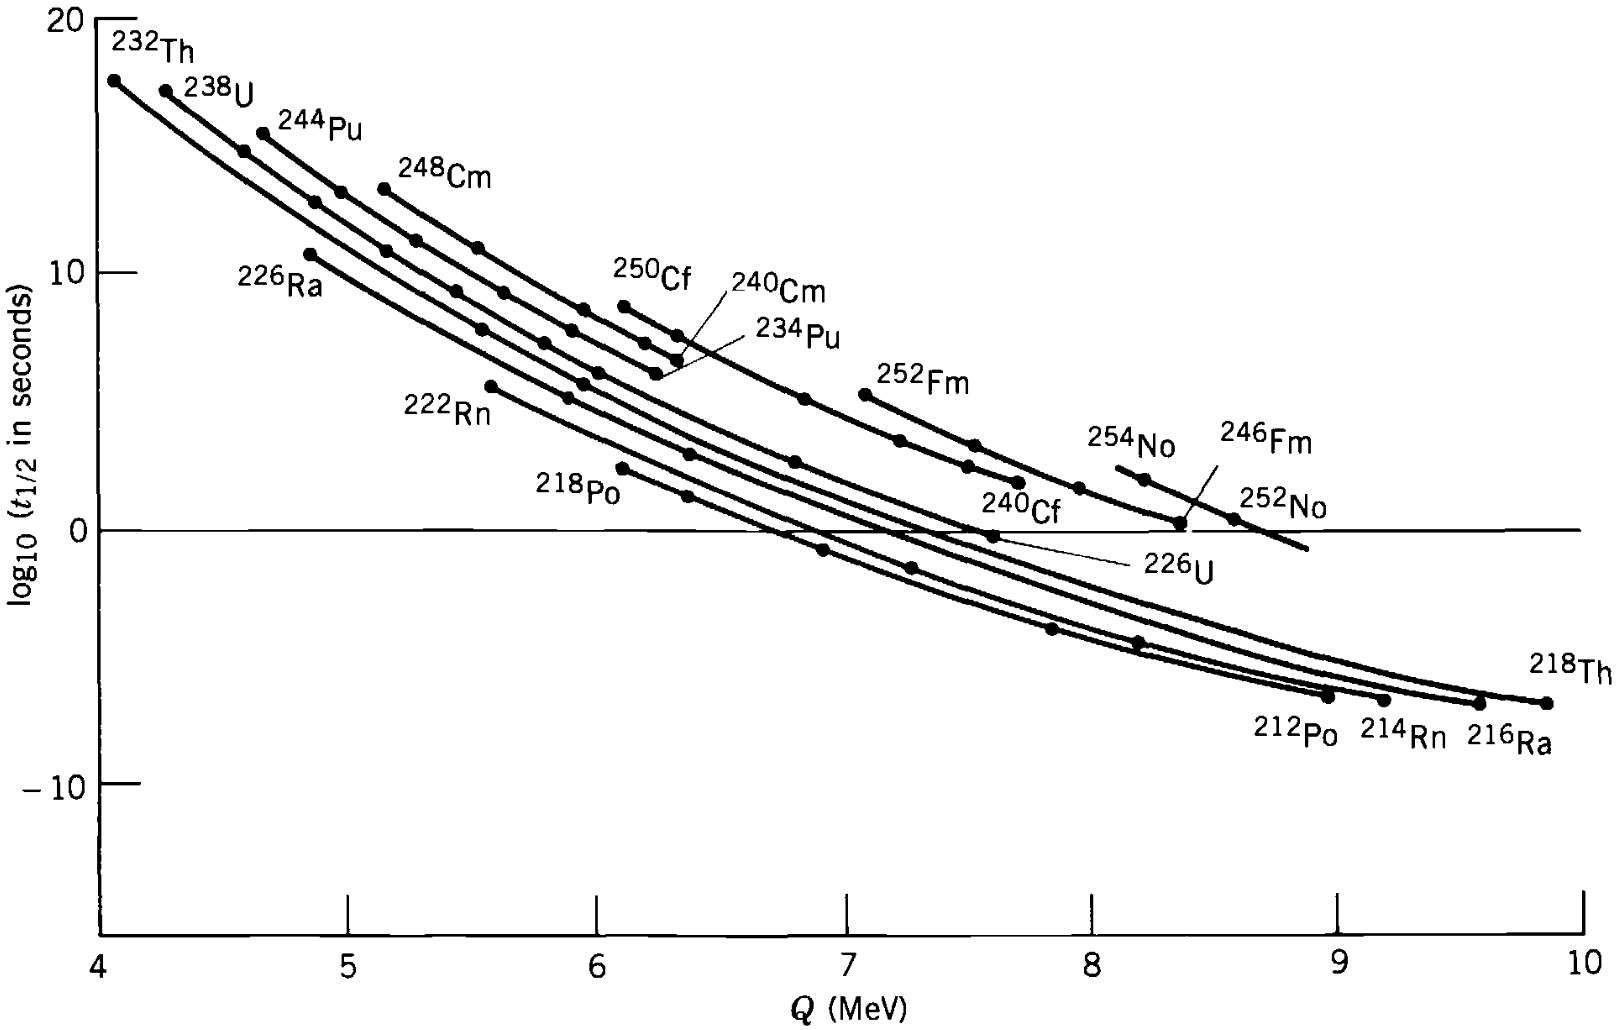
\includegraphics[width=0.50\textwidth]{geiger-nuttall.png}
	\caption{Legge di Geiger-Nuttal in famiglie isotopiche con nuclidi pari-pari.}
	\label{geiger-nuttall}
\end{figure}
\begin{figure}[!hb]
	\centering
	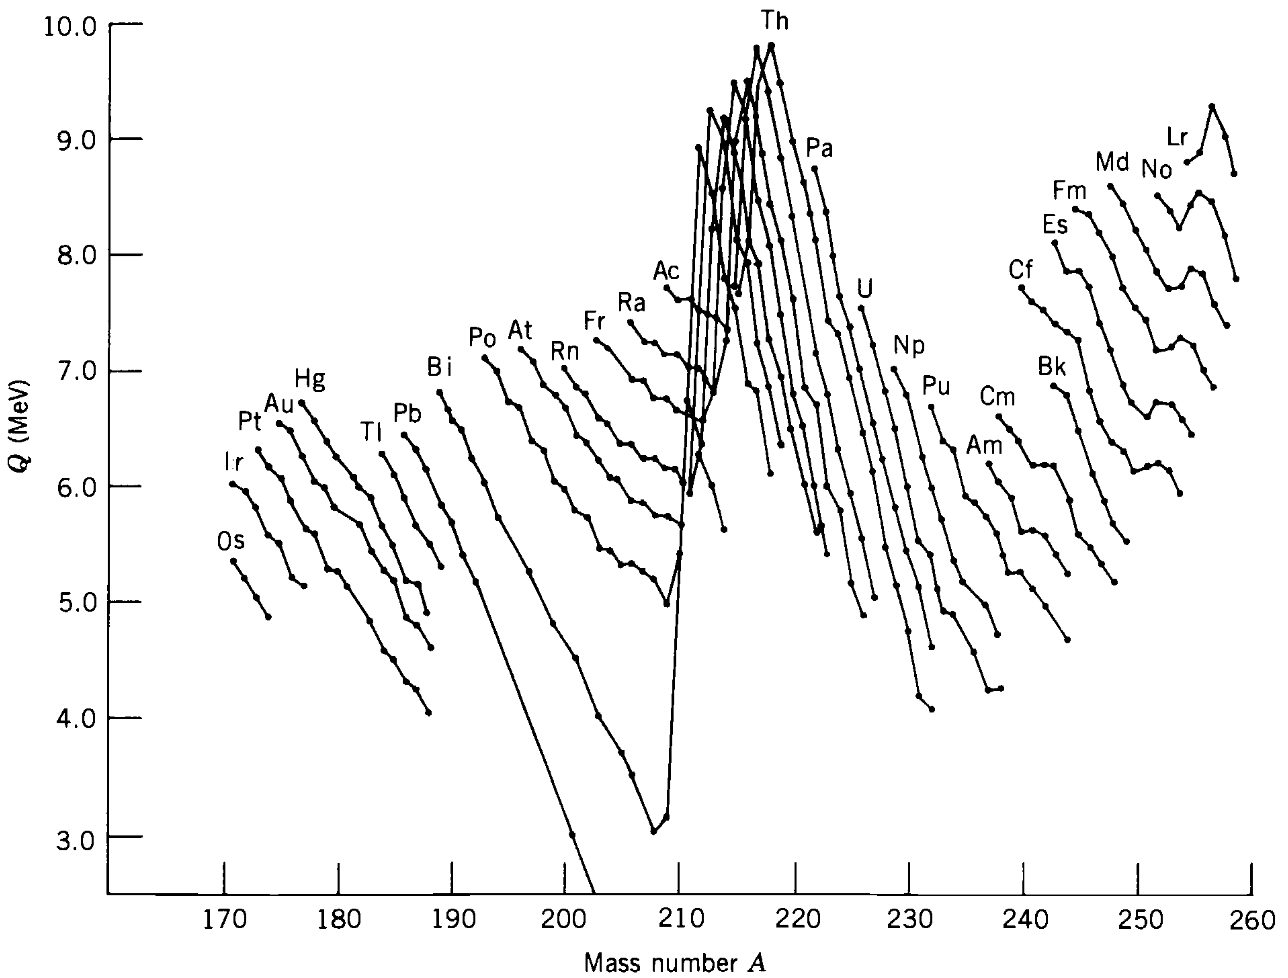
\includegraphics[width=0.50\textwidth]{gn-mass.png}
	\caption{Energia emessa per decadimento $ \alpha $ in famiglie isotopiche.}
	\label{gn-mass}
\end{figure}

\subsection{Teoria di Gamow}

La prima interpretazione teorica del decadimento $ \alpha $ fu data da Gamow nel 1929, qualche anno dopo le osservazioni di Geiger e Nuttall.\\
È possibile pensare alla particella $ \alpha $ come un corpo stabile preformato all'interno del nuclide $ \ch{^A X} $ che periodicamente di viene a trovare sulla superficie del nucleo, ad una distanza $ R \equiv R_{\ch{Y}} + R_{\alpha} $. Il moto della particella $ \alpha $ è determinato dal'energia potenziale d'interazione col nucleo, plottata in Fig. \ref{alpha-pot}, che fu proposta da Gamow essere:
\begin{equation}
	U(r) =
	\begin{cases}
		-V_0 & r < R \\
		\frac{2(Z-2)e^2}{4\pi \epsilon_0 r} & r > R
	\end{cases}
	\label{eq:2.12}
\end{equation}
con $ V_0 $ una costante positiva. Il senso fisico di tale espressione è che in prossimità del nucleo a prevalere è la forza nucleare, che ha natura attrattiva, mentre allontanandosi da esso prevale l'interazione coulombiana, che è repulsiva: si vede quindi la presenza di una barriera coulombiana in $ r = R $.\\
Con una trattazione classica la particella $ \alpha $ sarebbe emessa solo se $ E_{\alpha} > U(R) $ e ciò avverrebbe in un tempo comparabile al tempo di attraversamento del nucleo, ovvero $ t \sim R / v_{\alpha} = R \sqrt{2E_{\alpha} / m_{\alpha}} $: stimando $ R \approx 1.2\fm \left( (A - 4)^{1/3} + 4^{1/3} \right) $, per un nucleo con $ A \sim 230 $ e $ Q \sim 4\mev $ si trova $ R \sim 9\fm $ e $ t \sim 10^{-21}\,\text{s} $, ovvero un decadimento praticamente istantaneo. Ciò però non è quello che si osserva sperimentalmente.\\
Quantisticamente, invece, grazie all'effetto tunnel è possibile che anche le particelle $ \alpha $ con $ E_{\alpha} < U(R) $ (cosa che è praticamente sempre, dato che $ U(R) \sim 20\mev $) possono essere emesse con probabilità inderiori e dunque tempi di decadimento più lunghi.\\
È possibile svolgere il calcolo esplicitamente approssimando il potenziale coulombiano tra $ r = R $ ed $ r = R_{\alpha} $ (determinato da $ U(R_{\alpha}) = E_{\alpha} $) come una successione di barriere di potenziale di spessore $ dr $: dalla meccanica quantistica è noto che un'onda (particella) incidente su una barriera di potenziale di spessore $ L $ risulta in un'onda riflessa ed una trasmessa, le cui rispettive distribuzioni di probabilità (funzioni d'onda) sono determinate dai coefficienti di riflessione e trasmissione.

\begin{figure}[!hb]
	\centering
	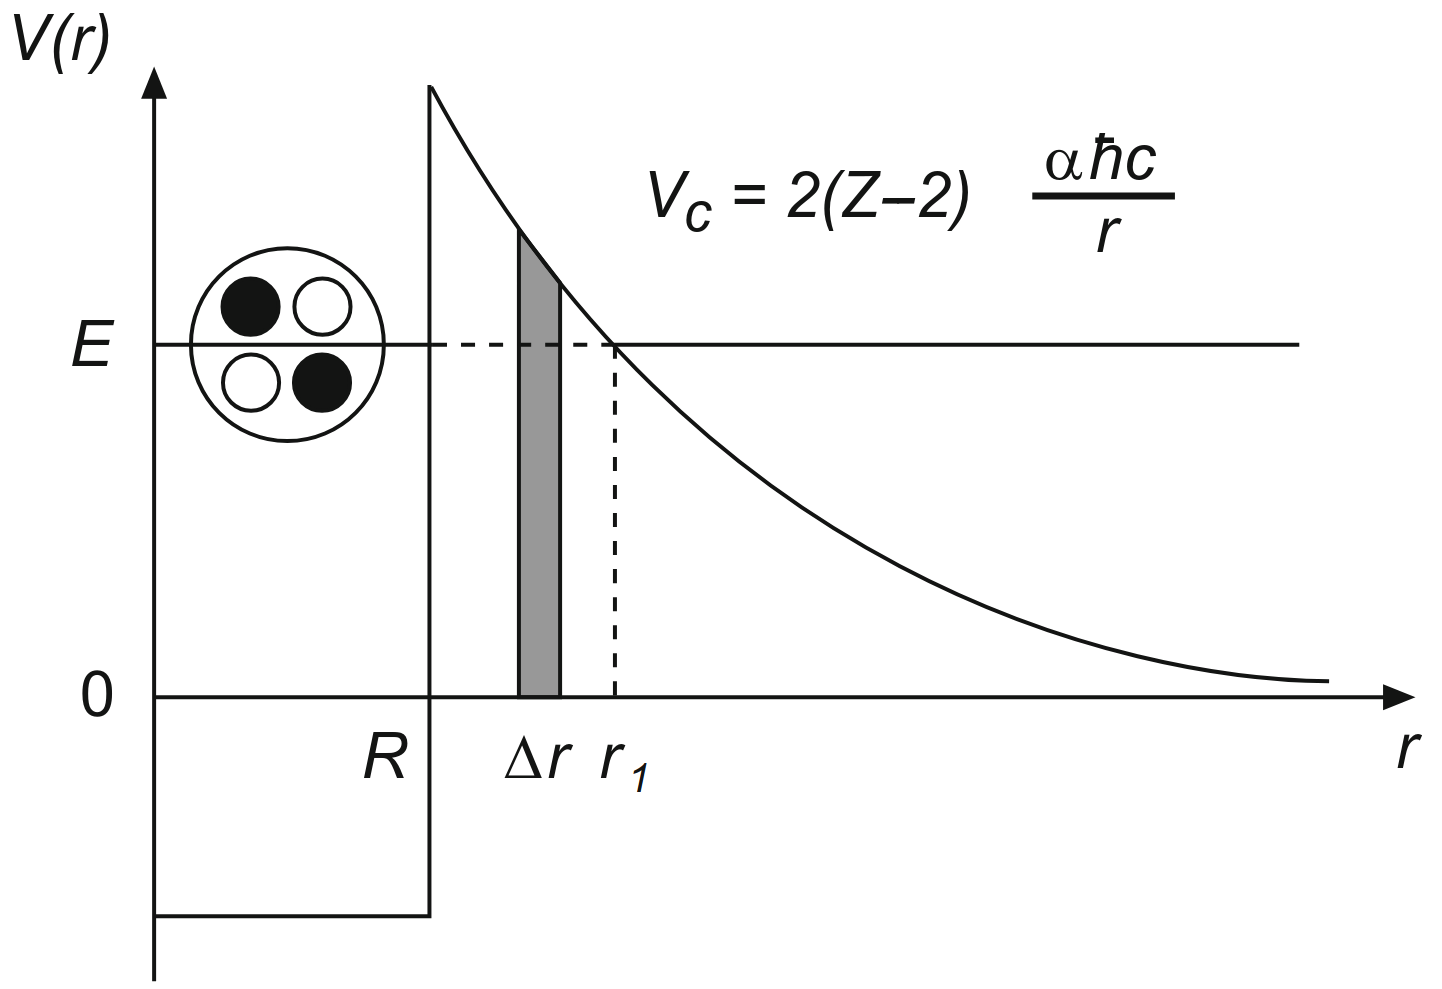
\includegraphics[width=0.60\textwidth]{alpha-pot.png}
	\caption{Potenziale d'interazione per il decadimento $ \alpha $.}
	\label{alpha-pot}
\end{figure}

Nel caso del decadimento $ \alpha $ è d'interesse solo il coefficiente di trasmissione nell'approssimazione $ E \ll V_0 $:
\begin{equation}
	T(E) = \left[ 1 + \frac{U_0^2}{4E (U_0 - E)} \sinh^2 \left( \frac{L}{\hbar} \sqrt { 2m (U_0 - E)} \right) \right]^{-1} \approx \frac{16 E (U_0 - E)}{U_0^2} e^{-2 \frac{L}{\hbar} \sqrt{2m (U_0 - E)}}
	\label{eq:2.13}
\end{equation}
Nel modello approssimato della successione di barriere di potenziale, quindi, si trova una probabilità di tunneling data da:
\begin{equation}
	P(E_{\alpha}) = \exp{\left[ -2 \int_{R}^{R_{\alpha}} dr \frac{1}{\hbar} \sqrt{2 m (U(r) - E_{\alpha}}) \right]} \eqdef e^{-2G}
	\label{eq:2.14}
\end{equation}
dove è stato definito il \textit{fattore di Gamow} $ G $. Svolgendo il calcolo col potenziale in Eq. \ref{eq:2.12} ed approssimando per una thick barrier $ R_{\alpha} \gg R $ (equivalente a $ E_{\alpha} \ll U(R) $, dato che dalla definizione $ R / R_{\alpha} = E_{\alpha} / U(R) $):
\begin{equation}
	\begin{split}
		G(E_{\alpha})
		&= \frac{2 (Z - 2) e^2}{\hbar} \sqrt{\frac{2m_{\alpha}}{E_\alpha}} \left[ \arccos \sqrt{\frac{R}{R_{\alpha}}} - \sqrt{\frac{R}{R_{\alpha}} - \frac{R^2}{R^2_{\alpha}}} \right]\\
		&\approx \frac{2 (Z - 2) e^2}{\hbar} \sqrt{\frac{2m_{\alpha}}{E_{\alpha}}} \left( \frac{\pi}{2} - \sqrt{\frac{R}{R_{\alpha}}} \right)
	\end{split}
	\label{eq:2.15}
\end{equation}
Questa espression mostra bene la fortissima dipendenza della probabilità di decadimento dall'energia della particella $ \alpha $: una piccola variazione di $ E_{\alpha} $ può portare $ P(E_{\alpha}) $ a variare di vari ordini di grandezza.\\
È anche possibile ricavare la legge di Geiger-Nuttall, dato che fenomenologicamente di può scrivere:
\begin{equation}
	\lambda = S \nu P(E_{\alpha})
	\label{eq:2.16}
\end{equation}
dove $ \lambda $ è la costante di decadimento, $ S $ è la probabilità che si formi una particella $ \alpha $ nel nucleo (può essere presa $ S \approx 1 $) e $ \nu $ è la knocking frequency, ovvero la frequenza con cui la particella $ \alpha $ urta con la barriera coulombiana. Si può stimare $ \nu $ a partire dal tempo che impiega la particella $ \alpha $ ad attraversare il nucleo (già trovato in precedenza): $ \nu \sim t^{-1} \sim 10^{21} \,\text{Hz} $. Dall'Eq. \ref{eq:2.16} si ha:
\begin{equation}
	\ln \lambda = \ln S + \ln \nu - 2 G(E_{\alpha}) \sim a(Z) - b \frac{Z}{\sqrt{E_{\alpha}}}
	\label{eq:2.17}
\end{equation}
che, ricordando che $ t_{1/2} = \frac{\ln 2}{\lambda} $, è proprio la legge di Geiger-Nuttall.\\
Ovviamente tutte queste relazioni sono qualitative e non quantitative, dato che sono state fatte alcune approssimazioni dalle quali la realtà si discosta notevolmente, prima su tutti la simmetria sferica: i nuclidi pesanti hanno forme notevolmente deformate (tendenti ad ellissoidi di rotazione), dunque le loro emissioni presentano notevoli anisotropie nella distribuzione angolare di particelle $ \alpha $.

\subsection{Spettri}

Per molti nuclidi che decadono tramite decadimento $ \alpha $ è possibile la presenza di più branch di decadimento, con percentuali di decadimento basse rispetto a quella dominante, che non portano direttamente allo stato fondamentale del nucleo figlio, ma a qualche suo stato eccitato: ciascuna di queste branch ha una propria energia di decadimento (deve essere sempre mono-energetico), e solitamente la branch con l'energia più alta è quella che va a popolare lo stato fondamentale del nucleo figlio.\\
Lo studio degli spettri di decadimento così prodotti (ad esempio immettendo le particelle $ \alpha $ in uno spettrometro magnetico) è importante per studiare i vari livelli energetici del nucleo figlio, specialmente nel caso in cui esso appartenga ad una specie nucleare di difficile sintesi.

\subsection{Cluster decay}

Spesso, quando un nuclide risulta instabile rispetto al decadimento per $ \ch{^4 He} $, esso lo è anche rispetto a quello per $ \ch{^8_4 Be} $, $ \ch{^{12}_6 C} $ ed altri nuclei, tendenzialmente formati da più particelle $ \alpha $, i cosiddetti \textit{nuclear clusters}. Anche questi sono sistemi particolarmente stabili preformati nel nucleo e, per un nuclear cluster di $ n $ particelle $ \alpha $, si può approssimare $ Q_n \sim Q_{\alpha}^n $: di conseguenza, per la legge di Geiger-Nuttall, i tempi di decadimento sono enormemente più lungi rispetto a quelli del decadimento $ \alpha $, con conseguenza che i branching ratios sono praticamente trascurabili, sebbene occasionalmente questi cluster decays vengano osservati e siano stati ampiamente studiati.










